\section{BraTS 2018 dataset}
The BraTS dataset \cite{menze2015multimodal} contains MRI scans of the human brain. It is provided by the University of Pennsylvania (U

\begin{figure}[H]
\centering
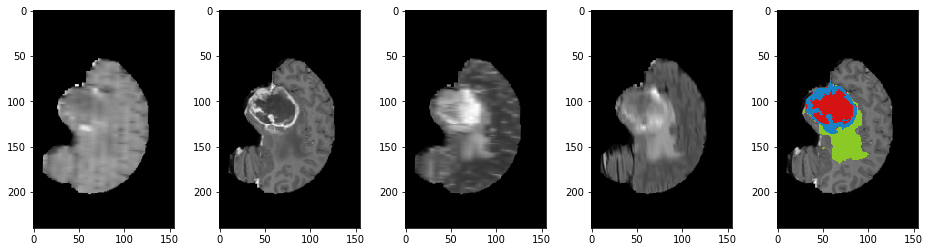
\includegraphics[width=14cm]{chapters/04_segmentation/images/brats.png}
\caption{One slice showing all 4 modalities and the tumor segmentation}
\end{figure}

\subsection{Ground truth/label}
The dataset contains a ground truth segment with the following tissue types:

\begin{itemize}
    \item Gadolinium-enhancing tumor (ET - label value 4)
    \item Peritumoral edema (ED - label value 2),
    \item Necrotic and non-enhancing tumor core (NCR/NET - label value 1)
\end{itemize}

The tissue types are explained in the next chapter.
